\begin{definition}[breakable]{Monotonie}\\
    Sei $y=f(x)$ eine differenzierbare Funktion in $D$ mit $x_{0} \in D$.
    \begin{itemize}
        \item $f'( x_{0}) = 0$ $ \Rightarrow$   $f$ konstant, bzw. horizontale Tangente
        \item $f'( x_{0}) > 0 $ $ \Rightarrow$  $f$  streng monoton wachsend.
        \item $f'( x_{0}) < 0 $ $ \Rightarrow$ $f$ streng monoton fallend.
    \end{itemize}
\end{definition}
\begin{theorem}{Krümmung}\\
    Zusammenhang zwischen 2. Ableitung und Krümmung:
    \begin{itemize}
      \item $f^{\prime \prime}\left(x_{0}\right)>0$ Konvex (Nach links/oben gekrümmt)
      \item $f^{\prime \prime}\left(x_{0}\right)<0$ Konkav (Nach rechts/unten gekrümmt)
      \item $f^{\prime \prime}\left(x_{0}\right)=0$ Keine eindeutige Krümmung
    \end{itemize}
    Bmk: Die Summe zweier konvexer Funktionen ist konvex. (konkav analog)
\end{theorem}

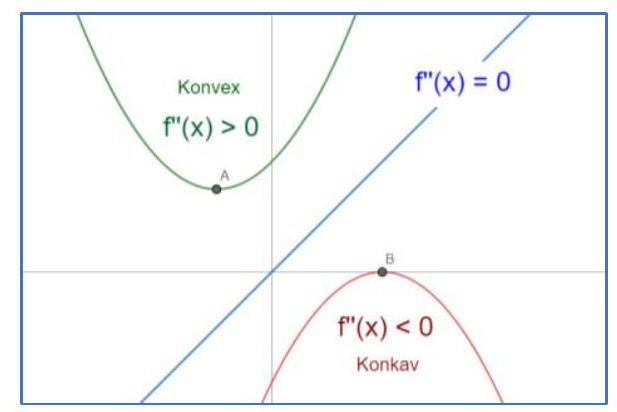
\includegraphics[scale=0.2]{Analysis1/zsf/Images/Integral/2024_01_20_7bfda6c084929ccc01ffg-07.jpg}
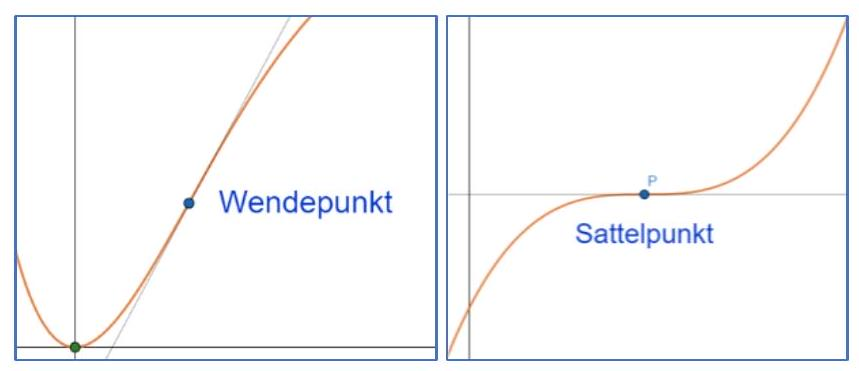
\includegraphics[scale=0.15]{Analysis1/zsf/sections/diff_funktionen/2024_01_20_7bfda6c084929ccc01ffg-08.jpg}
\begin{definition}{Wende- und Sattelpunkte}
    Als Wendepunkte werden Punkte bezeichnet bei denen sich der «Drehsinn» ändert. Wendepunkte mit horizontaler Tangente werden als Sattelpunkte oder Terrassenpunkte bezeichnet\\

Wendetangente:
\begin{itemize}
  \item Tangente an einem Wendepunkt
\end{itemize}
\end{definition}



\begin{KR}{Berechnung Wendetangente}
    Ermittlung durch Lösen der Gleichung $f^{\prime \prime}(x)=0 \rightarrow x_{0}$.\\
    Bedingungen:\\
    Sei $y=f(x)$ dreimal differenzierbar

\begin{itemize}
  \item $f^{\prime \prime}\left(x_{0}\right)=0$
  \item $f^{(3)}\left(x_{0}\right) \neq 0 \quad \rightarrow$ Wendepunkt
  \item Falls zusätzlich $f^{\prime}\left(x_{0}\right)=0 \quad \rightarrow$ Sattelpunkt
\end{itemize}
    
\end{KR}

\begin{concept}{Allgemeines Kriterium}\\
    Sei $f(x)$ eine genügend oft differenzierbare Funktion

\begin{itemize}
  \item $f^{\prime}\left(x_{0}\right)=0$
\end{itemize}

Sei $n$ die Ordnung der ersten nicht verschwindenden Ableitung von $f(x)$ an der Stelle $x_{0}$:

\begin{itemize}
  \item $f^{\prime}\left(x_{0}\right)=f^{\prime \prime}\left(x_{0}\right)=\cdots=f^{(n-1)}\left(x_{0}\right)=0$
  \item $f^{(n)}\left(x_{0}\right) \neq 0$
\end{itemize}

Schlussfolgerungen:
\begin{itemize}
    \item Wenn $n$ gerade, dann gibt es ein relatives Extremum $\left(f^{(n)}\left(x_{0}\right) \neq 0\right)$
    \item Wenn $n$ ungerade, dann hat $f(x)$ an der Stelle $x_{0}$ einen Wendepunkt und damit einen Sattelpunkt
\end{itemize}
\end{concept}

\begin{KR}{Vorgehen Wende- und Sattelpunkte}
    \begin{enumerate}
  \item Erste und zweite Ableitung

  \item Wendepunkt bestimmen

\end{enumerate}

\begin{itemize}
  \item $f^{\prime \prime}\left(x_{0}\right)=0 \rightarrow x_{0}$
  \item $f^{(3)}\left(x_{0}\right) \neq 0$
\end{itemize}

\begin{enumerate}
  \setcounter{enumi}{2}
  \item Sattelpunkte bestimmen
\end{enumerate}

\begin{itemize}
  \item $f^{\prime}\left(x_{0}\right)=0$
  \item $f^{\prime \prime}\left(x_{0}\right)=0$
  \item ...
  \item $f^{(n)}\left(x_{0}\right) \neq 0$
  \item Gerade $\rightarrow$ relatives Extremum
  \item Ungerade $\rightarrow$ Sattelpunkt
\end{itemize}

\begin{enumerate}
  \setcounter{enumi}{3}
  \item $x_{0}$ in ursprüngliche Gleichung einsetzen
\end{enumerate}
\end{KR}











